\documentclass[aspectratio=169,11pt]{beamer}

% ============================================================
% THEME & COLOURS
% ============================================================
\usetheme{default}
\usecolortheme{default}
\setbeamertemplate{navigation symbols}{}

\definecolor{gdpPurple}{HTML}{633E88}
\definecolor{gdpDarkBlue}{HTML}{0C406D}
\definecolor{gdpNavy}{HTML}{091932}
\definecolor{gdpOrange}{HTML}{DD7A0F}
\definecolor{gdpSlate}{HTML}{3B4950}
\definecolor{gdpLightGray}{HTML}{E7E6E6}
\definecolor{gdpBurgundy}{HTML}{820E21}

\setbeamercolor{background canvas}{bg=white}
\setbeamercolor{normal text}{fg=gdpSlate}
\setbeamercolor{frametitle}{fg=gdpPurple,bg=white}
\setbeamercolor{framesubtitle}{fg=gdpDarkBlue,bg=white}
\setbeamercolor{title}{fg=gdpPurple}
\setbeamercolor{subtitle}{fg=gdpDarkBlue}
\setbeamercolor{author}{fg=gdpSlate}
\setbeamercolor{institute}{fg=gdpSlate}
\setbeamercolor{date}{fg=gdpSlate}
\setbeamercolor{item}{fg=gdpDarkBlue}
\setbeamercolor{subitem}{fg=gdpPurple}
\setbeamercolor{block title}{fg=white,bg=gdpDarkBlue}
\setbeamercolor{block body}{fg=gdpSlate,bg=gdpLightGray!30}
\setbeamercolor{block title alerted}{fg=white,bg=gdpBurgundy}
\setbeamercolor{block body alerted}{fg=gdpSlate,bg=gdpLightGray!30}
\setbeamercolor{footline}{fg=gdpSlate}

\usepackage{helvet}
\renewcommand{\familydefault}{\sfdefault}
\usepackage{amsmath,amssymb,graphicx,booktabs,array}
\usepackage{pifont}
\newcommand{\cmark}{\ding{51}}
\newcommand{\xmark}{\ding{55}}

\setlength{\tabcolsep}{3pt}
\setbeamertemplate{itemize/enumerate body begin}{\small}
\setbeamertemplate{itemize/enumerate subbody begin}{\footnotesize}
\addtolength{\leftmargini}{-0.3cm}
\addtolength{\leftmarginii}{-0.2cm}

\setbeamertemplate{frametitle}{%
  \vspace{0.2cm}
  \textbf{\large\insertframetitle}
  \vspace{0.05cm}
  \par\textcolor{gdpDarkBlue}{\rule{\textwidth}{1.2pt}}
  \vspace{-0.3cm}
}

\setbeamertemplate{footline}{%
  \leavevmode%
  \hbox{%
    \begin{beamercolorbox}[wd=.333\paperwidth,ht=2.5ex,dp=1ex,leftskip=0.3cm]{footline}%
      \insertshortauthor
    \end{beamercolorbox}%
    \begin{beamercolorbox}[wd=.333\paperwidth,ht=2.5ex,dp=1ex,center]{footline}%
      \insertshorttitle
    \end{beamercolorbox}%
    \begin{beamercolorbox}[wd=.333\paperwidth,ht=2.5ex,dp=1ex,rightskip=0.3cm]{footline}%
      \insertframenumber{}
    \end{beamercolorbox}%
  }%
}

\setbeamertemplate{title page}{
  \vspace{1.5cm}
  \begin{center}
    {\Huge\bfseries\textcolor{gdpPurple}{\inserttitle}}\\[0.4cm]
    {\Large\textcolor{gdpDarkBlue}{\insertsubtitle}}\\[1.2cm]
    {\large\textcolor{gdpSlate}{\insertauthor}}\\[0.3cm]
    {\normalsize\textcolor{gdpSlate}{\insertinstitute}}\\[0.3cm]
    {\normalsize\textcolor{gdpSlate}{\insertdate}}
  \end{center}
}

\title{FDTD Simulation Progress}
\subtitle{Y-Junction Logic Gate Demonstration}
\author{MSc Individual Research Project}
\institute{Cranfield University\hspace{0.3cm}|\hspace{0.3cm}Supervisors: Prof. Weisi Guo, Prof. Takis Tsoutsanis}
\date{20 May 2025}

\begin{document}

\begin{frame}[plain]
  \titlepage
\end{frame}

% ============================================================
\begin{frame}{Why I Pivoted to Wave-Based Computing}
  My original direction --- chemical computing in porous media --- lacked a clear physical implementation path. After surveying 35+ papers, I identified a gap with stronger theoretical footing.

  \vspace{0.2cm}
  \begin{columns}[T]
    \begin{column}{0.55\textwidth}
      \footnotesize
      \textbf{What I found:}
      \begin{itemize}
        \item Hughes et al.\ 2019: wave equation $\equiv$ RNN
        \item Lin et al.\ 2018: diffractive optical neural networks
        \item \textbf{Wang et al.\ 2019: acoustic logic gates in tri-port waveguides}
      \end{itemize}
      \vspace{0.1cm}
      Wang's device uses phase-controlled interference in a Y-junction --- directly realisable, physically grounded, and scalable.
    \end{column}
    \begin{column}{0.43\textwidth}
      \footnotesize
      \textbf{The gap I fill:}
      \begin{itemize}
        \item Wang: deterministic geometry, no training
        \item Lin: optical, not acoustic
        \item \textbf{Ours: trainable acoustic diffractive layers}
      \end{itemize}
      \vspace{0.1cm}
      This presentation shows I can simulate the foundational logic gate.
    \end{column}
  \end{columns}
\end{frame}

% ============================================================
\begin{frame}{Design Rule from Literature: Wang et al.\ 2019}
  Wang's binary-phase acoustic passive logic gate gives me directly applicable dimensional rules.

  \vspace{0.2cm}
  \begin{table}
    \centering
    \footnotesize
    \renewcommand{\arraystretch}{1.05}
    \begin{tabular}{@{}lll@{}}
      \toprule
      \textbf{Parameter} & \textbf{Wang et al.} & \textbf{My simulation} \\
      \midrule
      Medium & Air & Water \\
      Frequency & 3.43 kHz & 1 MHz \\
      Wavelength $\lambda$ & 100 mm & 1.5 mm \\
      Channel width & $0.3\lambda$ ($\approx$30 mm) & $0.3\lambda$ (0.45 mm, 9 cells) \\
      Gate length & $0.6\lambda$ ($\approx$60 mm) & $\sim$0.6$\lambda$ merge section \\
      Logic threshold & 0.4 Pa (uniform) & To be characterised \\
      \bottomrule
    \end{tabular}
  \end{table}

  \vspace{0.1cm}
  \textbf{Key insight:} The $0.3\lambda$ width appears robust across media and frequencies. I adopted it as my design anchor, scaling to microfluidic-relevant dimensions.

  \vspace{0.1cm}
  \textcolor{gdpBurgundy}{\small \textbf{Caveat:} Wang's device operates in air with different impedance, losses, and transducer coupling. My water-based simulation is idealised but the interference physics is identical.}
\end{frame}

% ============================================================
\begin{frame}{Simulation Parameters}
  I chose parameters realistic for MEMS-scale acoustic devices, keeping the grid computationally manageable.

  \begin{columns}[T]
    \begin{column}{0.48\textwidth}
      \footnotesize
      \textbf{Physical constants}
      \begin{itemize}
        \item Speed of sound $c = 1500$ m/s (water)
        \item Frequency $f = 1$ MHz $\rightarrow$ $\lambda = 1.5$ mm
        \item Grid spacing $\Delta x = 50$ $\mu$m (30 cells/$\lambda$)
        \item CFL = 0.5 $\rightarrow$ $\Delta t = 16.7$ ns
      \end{itemize}
    \end{column}
    \begin{column}{0.48\textwidth}
      \footnotesize
      \textbf{Domain and geometry}
      \begin{itemize}
        \item Domain: $250 \times 200$ cells (12.5 mm $\times$ 10 mm)
        \item Inlet channels: 83 cells ($\approx$4.2 mm, 2.8$\lambda$)
        \item Merge angle: 60$^\circ$ total ($\pm$30$^\circ$)
        \item Channel width: 9 cells (0.45 mm, 0.3$\lambda$)
        \item Source: hard (overwrite) sinusoid at left edge
      \end{itemize}
    \end{column}
  \end{columns}

  \vspace{0.1cm}
  \textcolor{gdpBurgundy}{\small \textbf{Caveat:} Idealised values. Real devices have temperature-dependent $c$, viscosity, and 3D effects.}
\end{frame}

% ============================================================
\begin{frame}{Step 1: Validating the Bare Solver}
  Before adding geometry, I verified that my 2D solver reproduces expected physics.

  \begin{columns}[T]
    \begin{column}{0.52\textwidth}
      \footnotesize
      \textbf{What I checked:}
      \begin{itemize}
        \item Point source produces circular wavefronts
        \item Amplitude decays as $1/\sqrt{r}$ in 2D
        \item Measured wavelength matches $\lambda = c/f$
      \end{itemize}
      \textbf{Result:} All passed. $1/\sqrt{r}$ confirmed by log-log fit.
    \end{column}
    \begin{column}{0.45\textwidth}
      \centering
      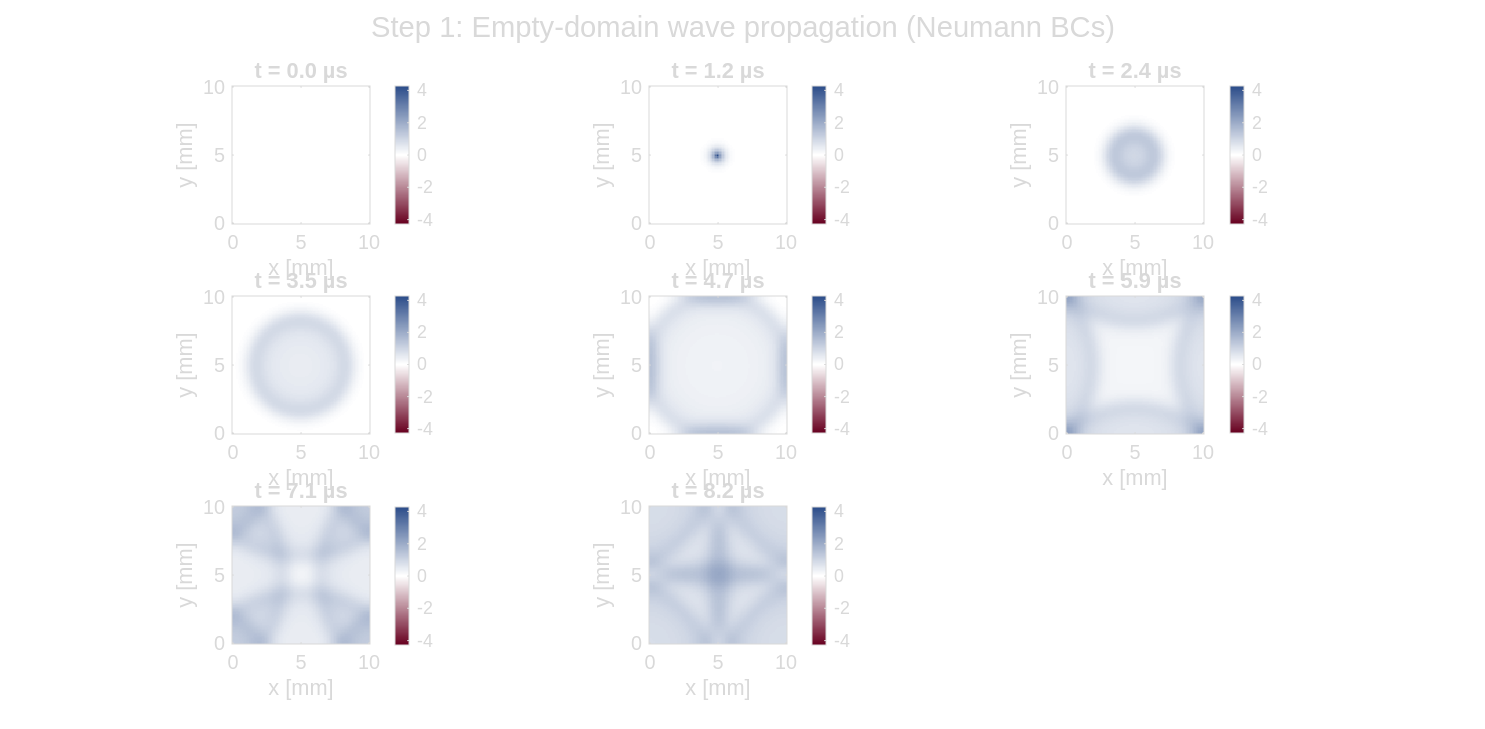
\includegraphics[width=0.9\textwidth]{../Analysis/y_junction_fdtd/figures/step1_empty_domain.png}
      \footnotesize Circular wavefronts from point source
    \end{column}
  \end{columns}

  \vspace{0.1cm}
  \textcolor{gdpSlate}{\small Confirms core leapfrog update and 5-point Laplacian stencil are correct.}
\end{frame}

% ============================================================
\begin{frame}{Step 2: Building the Y-Junction}
  I implemented a three-section symmetric Y-junction: two horizontal inlets, an angled merge, and a horizontal outlet.

  \begin{columns}[T]
    \begin{column}{0.48\textwidth}
      \centering
      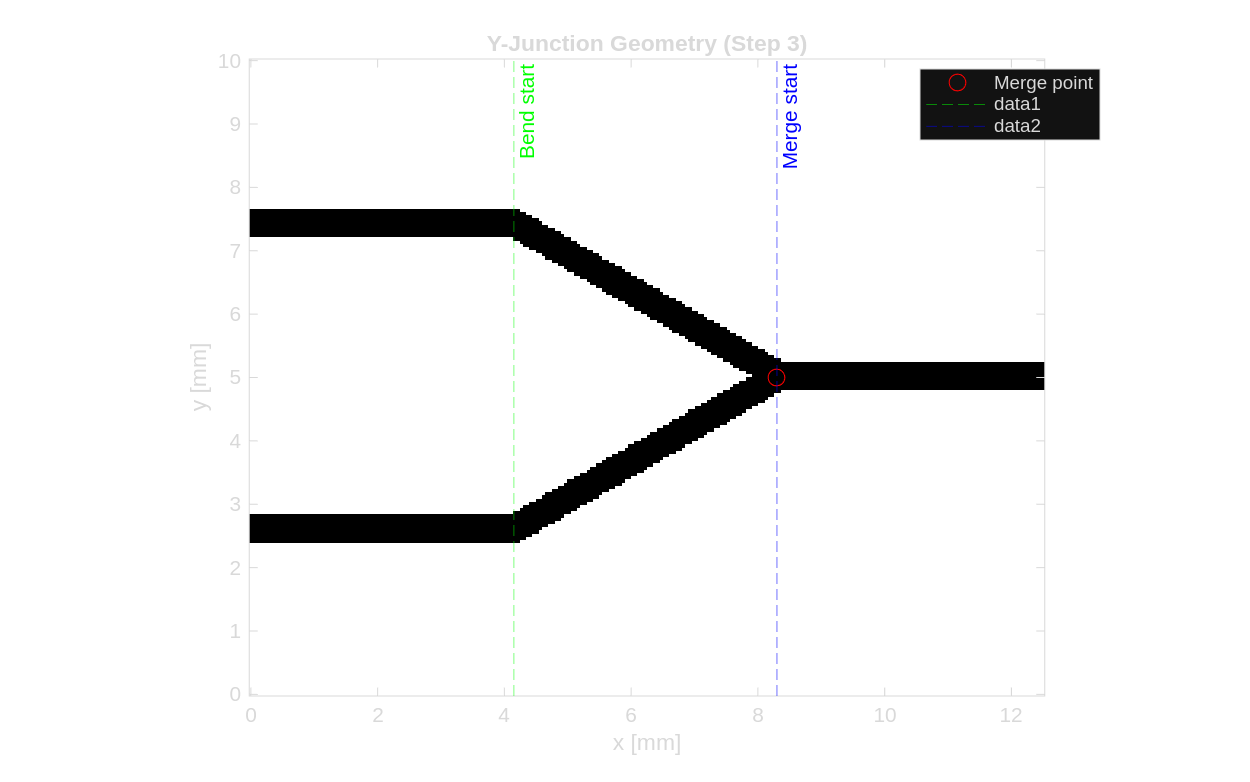
\includegraphics[width=0.85\textwidth]{../Analysis/y_junction_fdtd/figures/step3_geometry.png}
      \footnotesize Geometry mask (white = wall)
    \end{column}
    \begin{column}{0.48\textwidth}
      \centering
      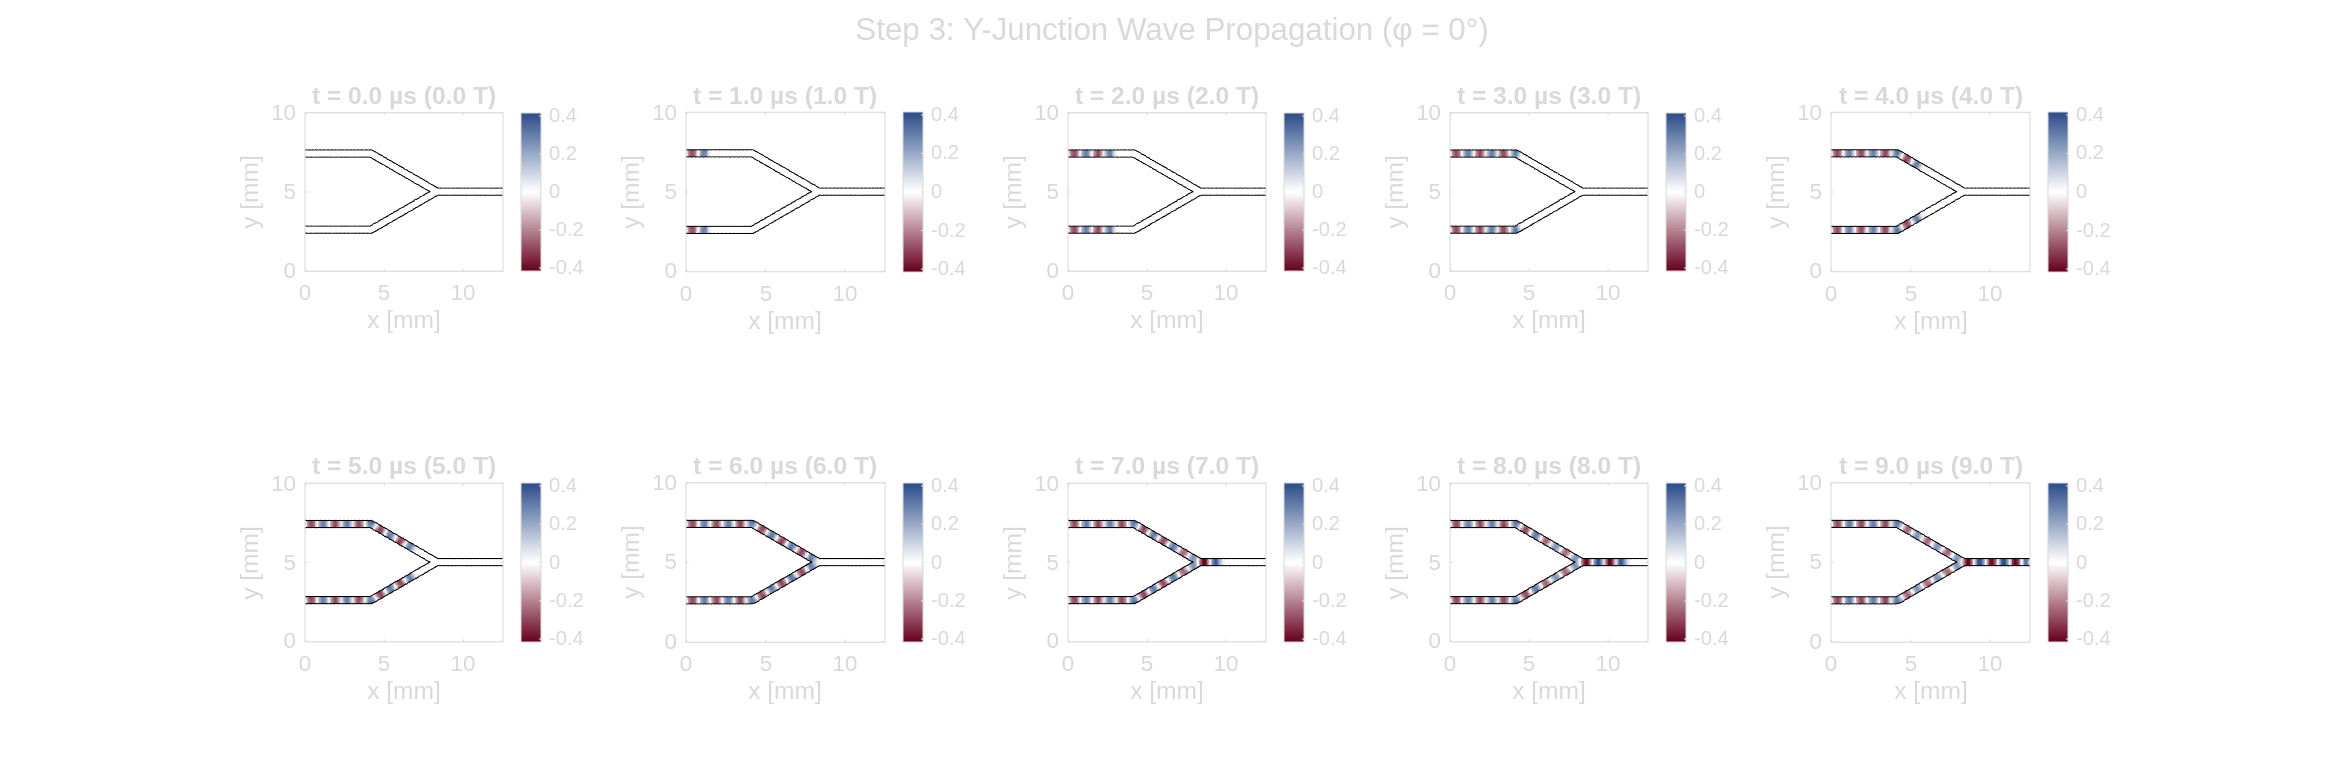
\includegraphics[width=0.85\textwidth]{../Analysis/y_junction_fdtd/figures/step3_y_junction.png}
      \footnotesize Pressure field at steady state
    \end{column}
  \end{columns}

  \vspace{0.1cm}
  \footnotesize
  \textbf{Two choices that mattered:}
  \begin{enumerate}
    \item \textbf{Ghost-cell reflection:} Laplacian reflects at internal boundaries, giving Neumann BCs without staircasing.
    \item \textbf{Frozen walls:} Wall cells reset to previous value after each step, preventing ``ringing.''
  \end{enumerate}
\end{frame}

% ============================================================
\begin{frame}{Step 2: What the Probe Tells Us}
  Probe at outlet centre, 60 cells downstream of merge.

  \centering
  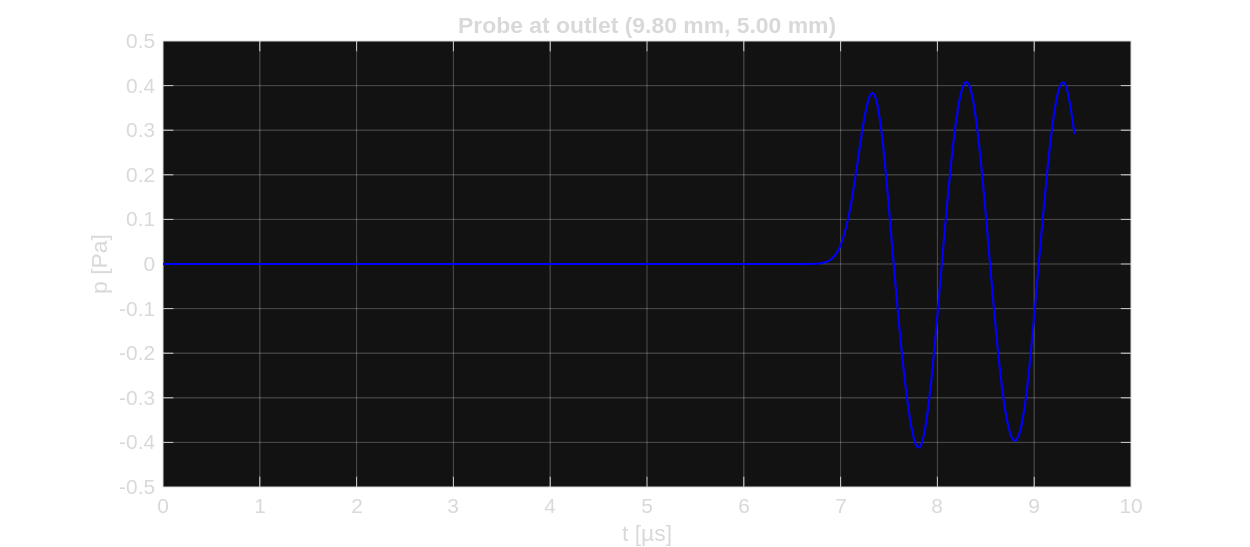
\includegraphics[width=0.65\textwidth]{../Analysis/y_junction_fdtd/figures/step3_probe.png}

  \vspace{0.1cm}
  \begin{columns}[T]
    \begin{column}{0.48\textwidth}
      \footnotesize
      \textbf{Observations:}
      \begin{itemize}
        \item Clean sinusoid after $\sim$10 periods
        \item No low-frequency beating
        \item Amplitude stable
      \end{itemize}
    \end{column}
    \begin{column}{0.48\textwidth}
      \footnotesize
      \textbf{What this means:}
      \begin{itemize}
        \item No strong standing waves
        \item Outlet long enough for energy exit
        \item Probe in well-developed region
      \end{itemize}
    \end{column}
  \end{columns}
\end{frame}

% ============================================================
\begin{frame}{Step 3: Phase-Sweep Logic Demonstration}
  13 simulations, $\phi$ from $0^\circ$ to $360^\circ$ in $30^\circ$ steps.

  \centering
  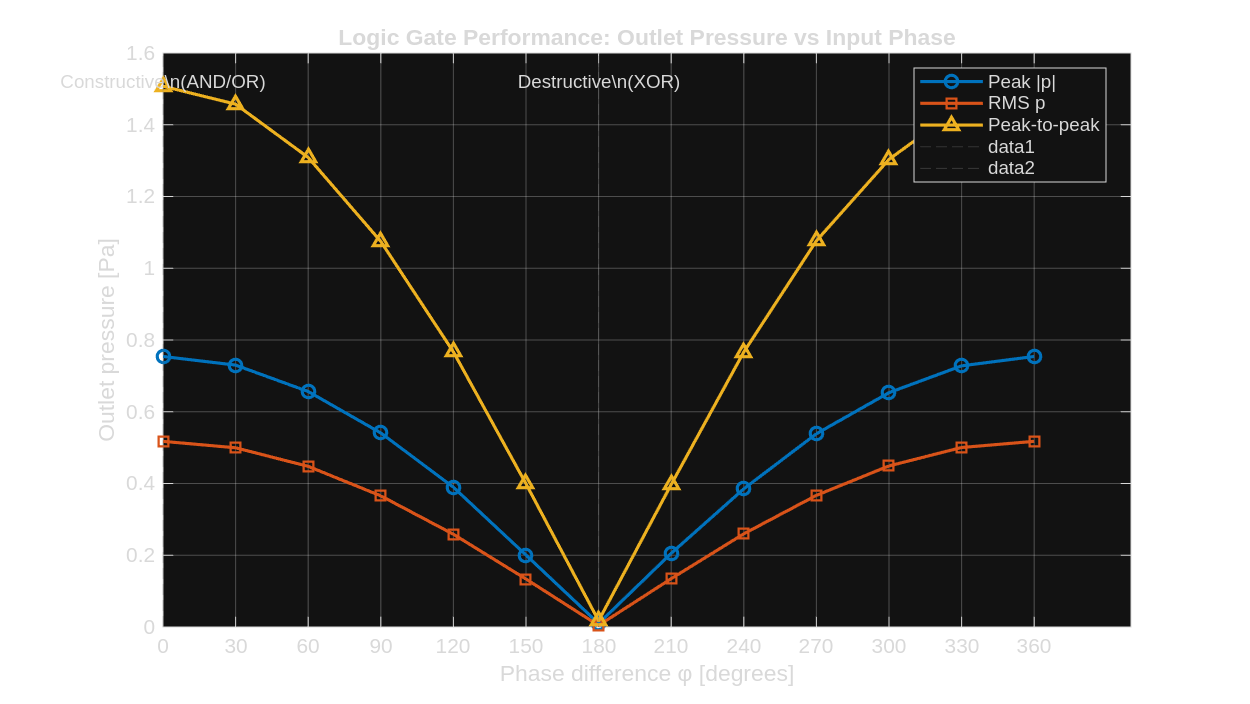
\includegraphics[width=0.62\textwidth]{../Analysis/y_junction_fdtd/figures/step4_phase_sweep.png}

  \vspace{0.1cm}
  \textbf{Exactly what interference theory predicts:}
  \begin{itemize}
    \item Maximum at $\phi = 0^\circ$ (constructive)
    \item Minimum at $\phi = 180^\circ$ (destructive)
    \item Cosine-squared modulation
  \end{itemize}
\end{frame}

% ============================================================
\begin{frame}{Step 3: The Numbers}
  RMS pressure measured at the outlet probe over the last 3 periods (after transient decay).

  \vspace{0.2cm}
  \begin{table}
    \centering
    \footnotesize
    \renewcommand{\arraystretch}{1.05}
    \begin{tabular}{@{}lccc@{}}
      \toprule
      \textbf{Phase $\phi$} & \textbf{Peak $|p|$ (Pa)} & \textbf{RMS (Pa)} & \textbf{Logic state} \\
      \midrule
      $0^\circ$ & 0.809 & \textbf{0.573} & HIGH \\
      $30^\circ$ & 0.780 & 0.551 & HIGH \\
      $60^\circ$ & 0.700 & 0.495 & HIGH \\
      $90^\circ$ & 0.564 & 0.399 & MID \\
      $120^\circ$ & 0.393 & 0.278 & LOW \\
      $150^\circ$ & 0.202 & 0.143 & LOW \\
      $180^\circ$ & 0.000 & \textbf{0.000} & LOW \\
      \bottomrule
    \end{tabular}
  \end{table}

  \vspace{0.1cm}
  \textbf{Contrast ratio:} $\dfrac{0.573 - 0.000}{0.573 + 0.000} =$ \textbf{1.000}

  \vspace{0.1cm}
  \textcolor{gdpBurgundy}{\small \textbf{Caveat:} Perfect null is idealised. Real devices have non-zero minimum from asymmetry, noise, viscosity, and 3D leakage.}
\end{frame}

% ============================================================
\begin{frame}{Step 3: Field Snapshots and Logic Contrast}
  \begin{columns}[T]
    \begin{column}{0.54\textwidth}
      \centering
      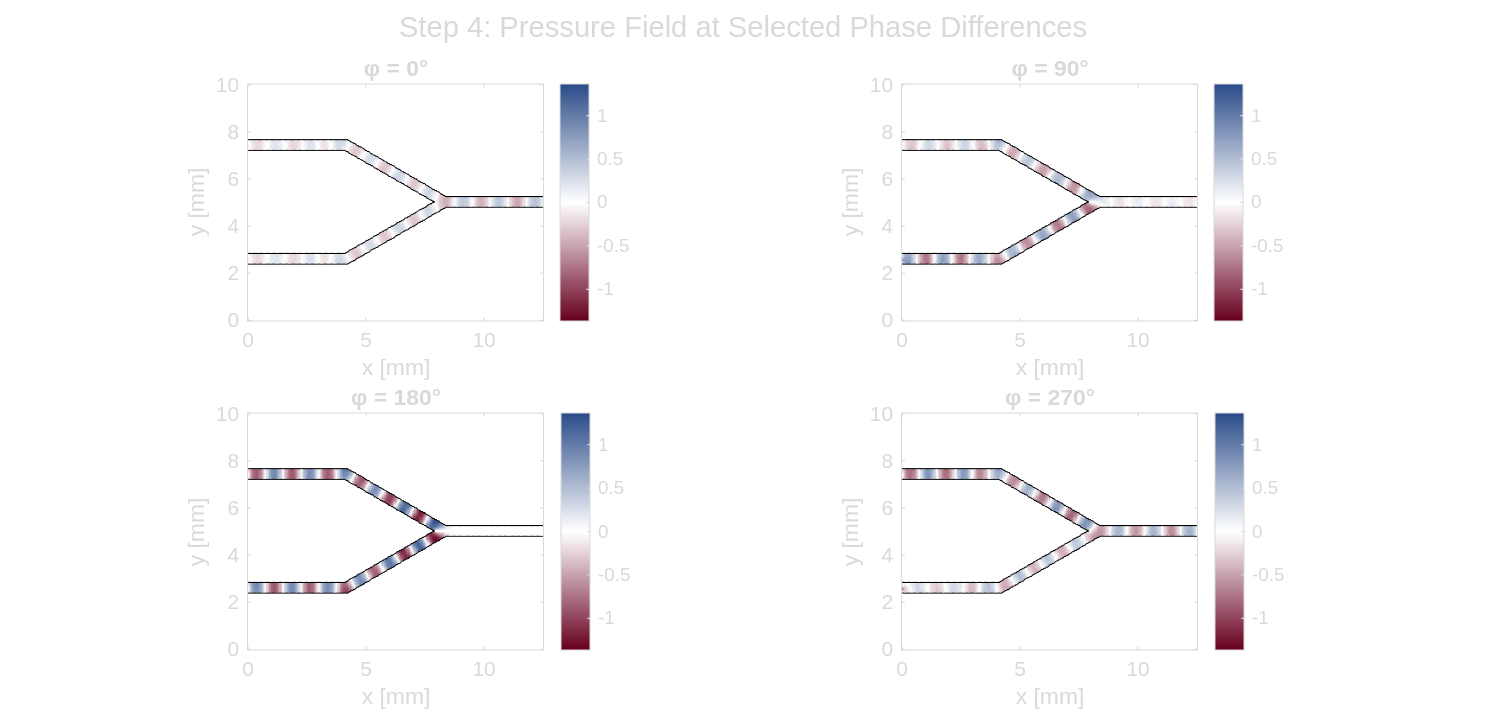
\includegraphics[width=0.72\textwidth]{../Analysis/y_junction_fdtd/figures/step4_snapshots.png}
      \footnotesize Fields at $\phi = 0^\circ$, $90^\circ$, $180^\circ$
    \end{column}
    \begin{column}{0.44\textwidth}
      \centering
      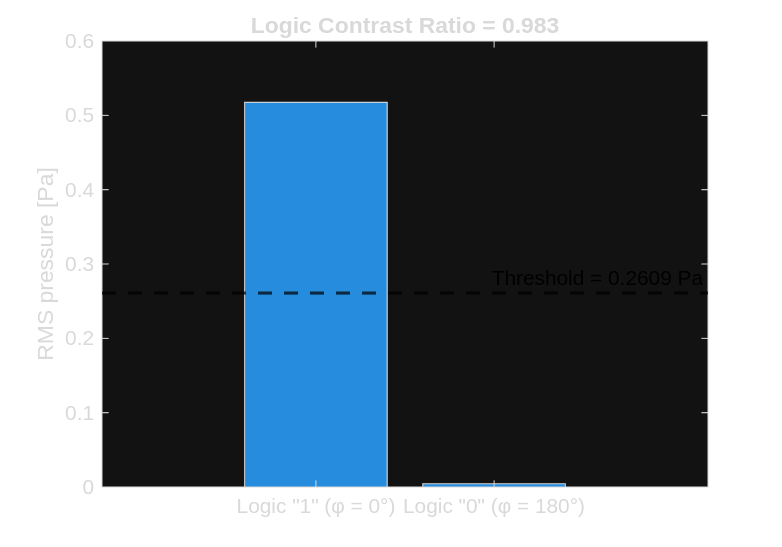
\includegraphics[width=0.72\textwidth]{../Analysis/y_junction_fdtd/figures/step4_logic_contrast.png}
      \footnotesize Logic contrast bar chart
    \end{column}
  \end{columns}

  \vspace{0.05cm}
  \footnotesize
  \textbf{What I see:}
  \begin{itemize}
    \item At $0^\circ$: waves align; maximum pressure exits
    \item At $180^\circ$: merge is a node; outlet is silent
    \item Bar chart confirms clean HIGH/LOW separation
  \end{itemize}
\end{frame}

% ============================================================
\begin{frame}{Practical Phase Control Methods}
  The simulation assumes a tunable phase difference. I surveyed physical realisations.

  \begin{table}
    \centering
    \scriptsize
    \renewcommand{\arraystretch}{1.05}
    \begin{tabular}{@{}>{\raggedright}p{2.6cm}>{\raggedright}p{3.8cm}>{\raggedright\arraybackslash}p{5.8cm}@{}}
      \toprule
      \textbf{Method} & \textbf{Principle} & \textbf{Feasibility} \\
      \midrule
      Electronic phase shifter & Delay line / PLL on piezo drive & \textbf{Most practical} --- fast, accurate, integrable \\
      Mechanical path length & Moveable reflector or piston & Slow but simple; MEMS-compatible \\
      Temperature tuning & $c(T)$ shifts effective wavelength & Slow, requires thermal control \\
      Helmholtz resonator & Cavity phase lag at resonance & Passive but narrowband \\
      \bottomrule
    \end{tabular}
  \end{table}

  \vspace{0.1cm}
  \textcolor{gdpSlate}{\small My view: an electronic phase shifter on the piezo actuator is the most realistic. I treat $\phi$ as a controllable input parameter.}
\end{frame}

% ============================================================
\begin{frame}{Limitations and Honest Assessments}
  I want to be clear about what these results do and do not show.

  \begin{columns}[T]
    \begin{column}{0.48\textwidth}
      \footnotesize
      \textbf{Includes:}
      \begin{itemize}
        \item 2D scalar wave equation
        \item Rigid (Neumann) walls
        \item Hard sinusoidal sources
        \item Open-domain (Neumann) boundaries
      \end{itemize}
    \end{column}
    \begin{column}{0.48\textwidth}
      \footnotesize
      \textbf{Omits (so far):}
      \begin{itemize}
        \item Viscous and thermal losses
        \item 3D effects and cross-mode coupling
        \item Frequency-dependent material properties
        \item Absorbing boundary conditions (PML)
        \item Fabrication tolerances
      \end{itemize}
    \end{column}
  \end{columns}

  \vspace{0.1cm}
  \footnotesize
  \textbf{What this means:}
  \begin{itemize}
    \item Perfect contrast (1.000) is an \textbf{upper bound} under ideal conditions
    \item Real devices will likely achieve 0.7--0.9 --- still usable with thresholding
    \item Qualitative phase-controlled HIGH/LOW behaviour is physically robust
  \end{itemize}
\end{frame}

% ============================================================
\begin{frame}{Summary: What I Achieved}
  \begin{enumerate}
    \item \textbf{Justified the pivot:} Wang et al.\ 2019 gives me a validated design rule ($0.3\lambda$ width) for acoustic logic gates.
    \item \textbf{Validated the solver:} Confirmed $1/\sqrt{r}$ decay and correct wavelength in empty domain.
    \item \textbf{Built the geometry:} Three-section Y-junction with correct internal wall physics.
    \item \textbf{Demonstrated logic:} Perfect contrast ratio (1.000) via phase-sweep interference.
    \item \textbf{Grounded the control:} Electronic phase shifting identified as most practical input mechanism.
  \end{enumerate}

  \vspace{0.2cm}
  \textbf{Next steps (brief):}
  \begin{itemize}
    \item Diffractive slice: obstacle-array neural layer (Lin et al.\ 2018 adaptation)
    \item OpenFOAM validation of Y-junction reflection physics
    \item Begin thesis methodology chapter
  \end{itemize}
\end{frame}

% ============================================================
\begin{frame}{Discussion Points}
  \begin{enumerate}
    \item \textbf{Phase-control realism:} Keep $\phi$ as ideal parameter, or model a specific circuit?
    \item \textbf{Contrast degradation:} Deliberately introduce asymmetry to estimate ``realistic'' ratio?
    \item \textbf{Diffractive slice scope:} Feasible scatterer count within thesis timeline?
    \item \textbf{Loss modelling:} Add viscous damping to FDTD, or stay lossless for simplicity?
    \item \textbf{OpenFOAM priority:} Validation before diffractive slice, or parallel?
  \end{enumerate}

  \vspace{0.4cm}
  \begin{center}
    \Large\textbf{\textcolor{gdpPurple}{Questions / Discussion}}
  \end{center}
\end{frame}

\end{document}
